\documentclass[10pt,a4paper]{article}
\usepackage[utf8]{inputenc}
\usepackage{amsmath}
\usepackage{amsfonts}
\usepackage{amssymb}
\usepackage{tikz}
\usepackage{graphicx}
\author{James Lee}
\title{4th Assignment of Computational Physics}
\begin{document}
	\maketitle
	\begin{abstract}
		In this report I present to you the numerical solution to Problem 1.3. As the procedures are quite trivial, I will spend more time in exploring the package \emph{Matplotlib}.
	\end{abstract}
	\section{Main Content}
	This program aims to calculate a ball's vertical motion when friction cannot be ignored.\\
	As a useful approximation, we consider the friction to have linear relation with velocity;
	\begin{equation}
    f_{\mu}=-\gamma v_{y}
	\end{equation}
	Assuming the initial velocity is against graity.\\
	Analysis of forces presented:\\
	\begin{center}
		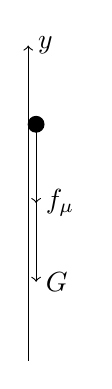
\begin{tikzpicture}
		\draw [->] (0,0) --(0,4);
		\draw [fill] (0.1,3) circle[radius=0.1];
		\draw [->] (0.1,3) --(0.1,1);
		\node [right] at (0.1,1) {$G$};
		\draw [->] (0.1,3) --(0.1,2);
		\node [right] at (0.1,2) {$f_{\mu}$};
		\node [right] at (0,4) {$y$};
		\end{tikzpicture}
	\end{center}
	According to Newton's 2nd Law, the dynamical equation is:
	\begin{align}
	m\frac{dv_y}{dt}&=-G+f_{\mu} \nonumber \\
	                &=-G-\gamma v_y
	\end{align}
	Set $m=1kg$, $G=mg=10N$.
	\subsection{$v_0=10m/s$ with $\gamma=1kg /s$}
	Easy to obtain the analytical soultion:
	\begin{equation}
	v=\frac{10\gamma+10}{\gamma} e^{-\gamma t}-\frac{10}{\gamma}
	\end{equation}
	Now we wish to exploit the numerical method to solve the equation.\\
	By using Euler method, we are able to convert ODE to difference equation. In terms of this idea, we have:
	\begin{equation}
	m\frac{v_y(t+\tau)-v_y(t)}{\tau}=-G-\gamma v_y(t)
	\end{equation}
	Given $v_y(0)$, we are able to obtain a set of discrete values of $v_y(t)$ using Euler method.\\
	Apparently, the smaller $\tau$ is, the more accurate our result will be.\\
	The figure shown below is our numerical solution:\\
	\begin{figure}[htbp]
		    \centering
			\includegraphics[width=5in]{Solution.png}
			\caption{Numerical Solutions with different $\tau$}
	\end{figure}
    As we can see, deviation from theoretical result is quite large when $\tau=1s$. This deviation begins to decrease as $\tau$ gets smaller. When $\tau=0.1s$, the numerical solution is quite good.
	
    \subsection{$v_0=10m/s$ with different $\gamma$}
    Intuitively, if friction is large, this ball will accerlerate to the saturated velocity.\\
    Thus, I will pick different numerical value of $\gamma$ to test this intuition.\\
    Note that following numerical solution are obtained under the condition $\tau=0.05s$.
    The figure shown below is our numerical solution:\\
     \begin{figure}[htbp]
     	\centering
     	\includegraphics[width=5in]{Solution_2.png}
     	\caption{Numerical Solution with different $\gamma$}
     \end{figure}
    In our figure, red curve is the friction-free case. As we can see, if $\gamma$ gets smaller, the shape of the curve will become nearer to the friction-free curve.\\
    Another thing to notice is that the numerical value of $\gamma$ will affect the saturation velocity. This property can be understood through analytical solution.
    
    \section*{Acknowledgement}
    When tackling this assignment, I benefitted a lot from the valuable discussions with Liu Xingchen. I would like to thank him for pointing out several grammar errors I made, also, for his willingness to discuss with me.
    
    \begin{thebibliography}{99}
    	\bibitem{}Hunter J, the Matplotlib Documentation, 2016
    	\bibitem{}Giordano N.J, Nakanishi H, Computational Physics, Pearson Education, 2007
    \end{thebibliography} 
\end{document}